\section{Ensemble Design}
% motivation for creating this theme
\begin{frame}{Designing the Ensemble}{R-FCN ResNet-101}
    \begin{block}{Overview}
    \begin{itemize}
        \item Ensemble of R-FCNs with ResNet-101
    \end{itemize}
    \begin{enumerate}
        \item Data sampling \& selection
        \begin{itemize}
            \item Object resolution
            \item Image quality
        \end{itemize}
        \item Training member classifiers
        \begin{itemize}
            \item Kept constant
        \end{itemize}
        \item Combining ensemble members
        \begin{itemize}
            \item Average
            \item Weighted Average
        \end{itemize}       
    \end{enumerate}
\end{block}
\end{frame}

\begin{frame}{Designing the Ensemble}{Pipeline}
    \begin{figure}
        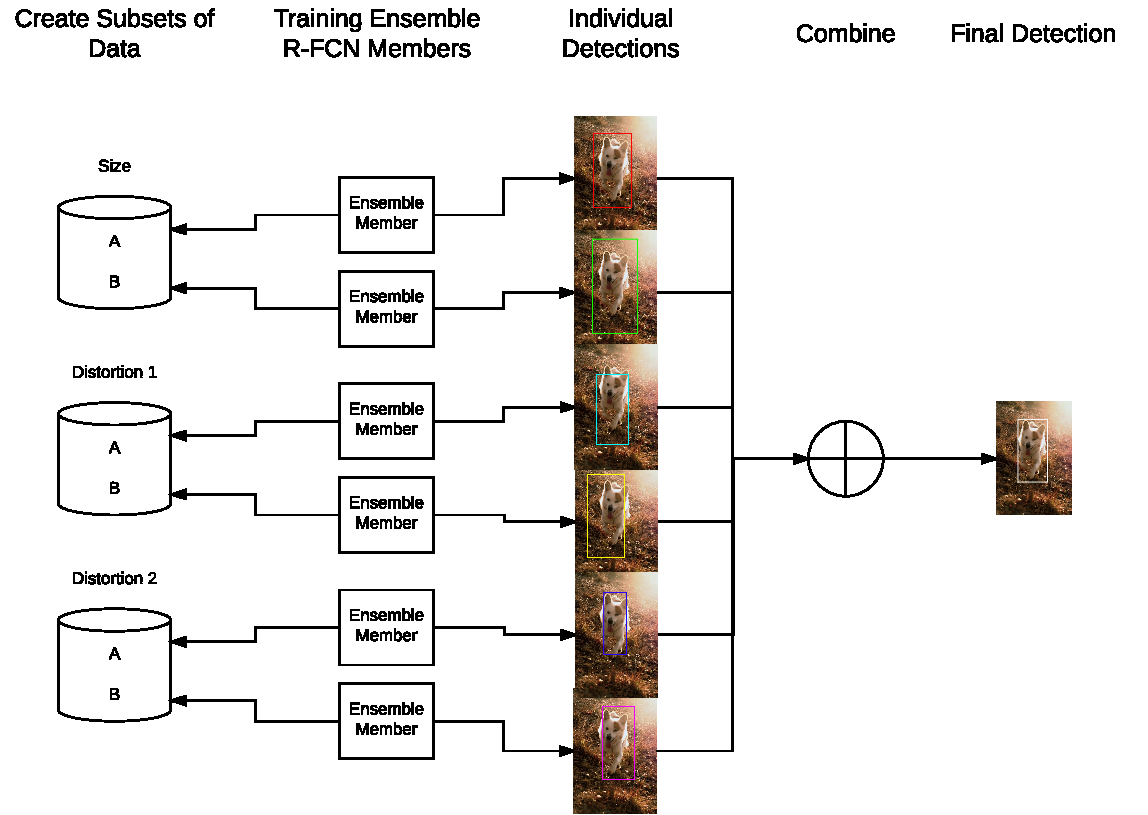
\includegraphics[width=0.8 \textwidth]{figs/ensembledesign.pdf}
    \end{figure}
\end{frame}

\begin{frame}{Training R-FCNs}{Ensemble Members}
\begin{columns}
    \column{0.5\textwidth}
        \begin{block}{Multi-step training}
        \begin{itemize}
            \item Train classifier with proposal inputs
            \item Ensure ensemble members infer from same input
            \item Simplify training process
        \end{itemize}
    \end{block}
    \column{0.5\textwidth}
        \begin{figure}
            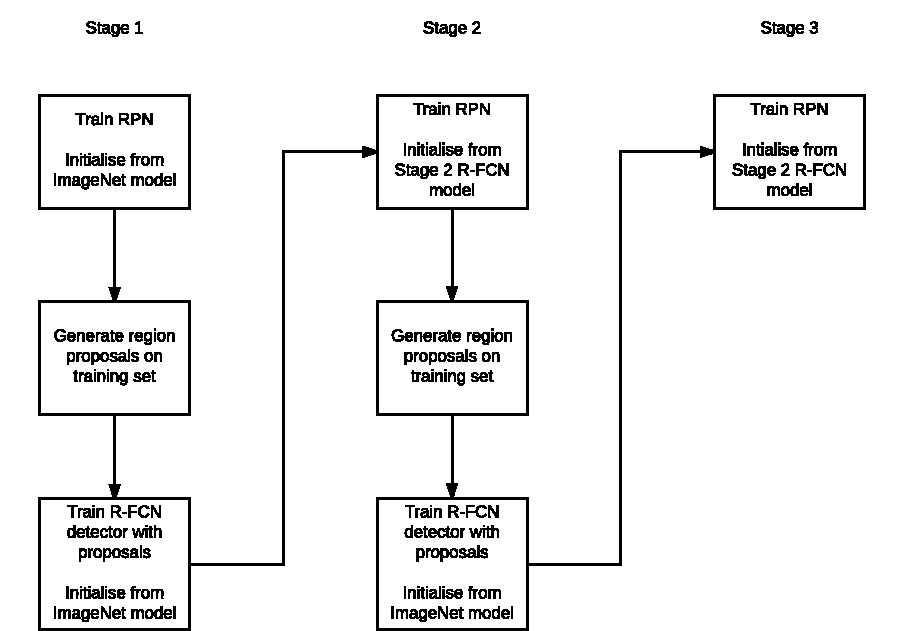
\includegraphics[width=1.0 \textwidth]{figs/4step-crop.pdf}
        \end{figure}
    \end{columns}
\end{frame}
